%!TEX root = ../template.tex
%%%%%%%%%%%%%%%%%%%%%%%%%%%%%%%%%%%%%%%%%%%%%%%%%%%%%%%%%%%%%%%%%%%%
%% chapter2.tex
%% NOVA thesis document file
%%
%% Chapter with the template manual
%%%%%%%%%%%%%%%%%%%%%%%%%%%%%%%%%%%%%%%%%%%%%%%%%%%%%%%%%%%%%%%%%%%%

\typeout{NT FILE chapter2.tex}%

\chapter{Direct Reactions as Spectroscopic Tools}
\label{cha:reactions}

\epigraph{
	"Nature hides her secrets because of her essential loftiness, but not by means of ruse."
}{Albert Einstein}

\epigraph{
	"The art of simplicity is a puzzle of complexity."
}{Douglas Horton}

%\glsresetall


\section{Introduction}
\label{sec:introduction}

The structure of atomic nuclei—how protons and neutrons arrange themselves in shells, how they correlate, and how these features evolve across the nuclear chart—has been at the heart of nuclear physics for decades. To unravel this structure, nuclear physicists have long relied on direct reaction mechanisms, in which a projectile interacts with a target nucleus in a controlled and selective way, producing clean signatures of specific internal configurations. Among these, transfer reactions and knockout reactions have historically provided the foundational experimental pathways for exploring the single-particle nature of the nucleus.


\section{Transfer Reactions}
\label{sec:transfer_reactions}

Nucleon transfer reactions, such as (d,p), (p,d), or (t,$\alpha$), involve the exchange of one or more nucleons between the projectile and the target. In the classic (d,p) reaction, for instance, a neutron is transferred from a deuteron to the target nucleus, leaving the residual system in a state that reveals the properties of the added neutron orbital.

These reactions have played a central role in defining the shell model: by measuring angular distributions and comparing them to reaction theory (e.g., using the distorted wave Born approximation, DWBA), one can extract:
\begin{itemize}
	\item The orbital angular momentum \emph{l} of the transferred nucleon (via angular distribution patterns).
	\item The spectroscopic factor, quantifying the overlap between the initial and final nuclear states.
\end{itemize}


Transfer reactions are best suited for stable or long-lived nuclei at relatively low energies (5–50 MeV/u), where they benefit from high cross-sections and well-developed theoretical frameworks. However, they become experimentally challenging for short-lived isotopes and high-Z systems, especially where targets cannot be fabricated.


\section{Knockout Reactions}

With the advent of radioactive beam facilities, transfer methods began to be complemented—and in some cases replaced—by nucleon knockout reactions, particularly in inverse kinematics. In a knockout reaction, such as (A, A–1), a high-energy projectile nucleus collides with a light target (e.g., $^2Be$, C, or H), and a single nucleon is suddenly removed from the projectile.

Knockout reactions operate in the sudden approximation: the interaction is fast enough that the removed nucleon doesn't reconfigure its wavefunction during the process. The resulting residual nucleus and its kinematics encode the structural information of the pre-existing configuration.

By measuring the momentum distribution of the residual fragment and comparing it with theoretical predictions (e.g., via the eikonal reaction model or Glauber theory), one obtains:

\begin{itemize}
	\item The \emph{l}-value of the knocked-out nucleon (from the width and shape of the distribution).
	\item The spectroscopic strength, linked to orbital occupancy.
\end{itemize}


Knockout reactions revolutionized structure studies of exotic nuclei, especially those near the drip lines, by enabling measurements of systems that could only be formed in-flight.

\section{From Knockout to Quasi-Free Scattering}

While both transfer and knockout reactions have yielded profound insights, their selectivity and interpretability face limitations. Transfer reactions are constrained by target availability and are often restricted to stable systems. Knockout reactions, although experimentally versatile, involve complex reaction dynamics with model dependencies that grow in neutron-rich environments and at higher energies.

To transcend these limitations, quasi-free scattering has re-emerged as a uniquely powerful probe. Conceptually close to knockout, but kinematically richer and theoretically cleaner in many regimes, quasi-free scattering reactions like (e,e'p) and (p,2p) offer direct access to the momentum and separation energy of individual nucleons in their initial nuclear orbitals. In high-energy kinematics, and under the impulse approximation, the scattering process isolates the interaction between the probe and a single nucleon, while the remaining nucleus acts as a spectator.

This progression—from transfer, to knockout, to quasi-free scattering—represents not just an evolution of experimental technique, but a deepening of our ability to map the quantum landscape inside the nucleus, from its shell structure to the underlying many-body correlations.


\section{Quasi-free Scattering Reactions}

\subsection{Introduction to Quasi-Free Scattering}

\gls{QFS} has emerged as one of the most powerful tools in nuclear physics to probe the single-particle structure and correlations within atomic nuclei. It encompasses a class of reactions in which an incident probe (either an electron or a proton) interacts predominantly with a single nucleon in the nucleus, while the remaining nucleons act as passive spectators. Under kinematic conditions favoring large momentum and energy transfer, and small final-state interactions (FSI), the process can be approximated by the impulse approximation (IA)—a simplification in which the nuclear many-body system is treated as a collection of quasi-free, independent nucleons.


\subsection{Historical Context and the Electron-Induced Paradigm}

The conceptual and experimental foundations of \gls{QFS} were established in the 1960s, particularly with the pioneering review by Jacob and Maris (1966) \cite{jacob_quasi-free_1966}, which systematized the theoretical framework for electron-induced \gls{QFS} reactions of the type (e,e'p). In these reactions, a high-energy electron transfers a well-defined amount of momentum and energy to a proton within the target nucleus, which is then ejected and detected in coincidence with the scattered electron. The kinematic constraints of such experiments enable the reconstruction of the missing energy and momentum of the ejected nucleon, which provides a direct spectroscopic window into the bound-state wavefunction.

This formalism was further refined in the 1973 follow-up by the same authors \cite{jacob_quasi-free_1973}, which accounted for distortions in both the incoming and outgoing waves due to the nuclear potential—introducing the Distorted Wave Impulse Approximation (DWIA). These early (e,e'p) experiments, primarily conducted at SLAC and Saclay, provided critical benchmarks for understanding shell structure, spectroscopic factors, and occupancy probabilities, particularly in medium-mass nuclei like $^{16}$O and $^{40}$Ca. However, the method remained largely confined to stable nuclei due to the limitations in electron beam-target combinations.


\subsection{Proton-Induced QFS and DWIA Evolution}

In parallel, the use of proton-induced \gls{QFS}—such as (p,2p) or (p,pn) reactions—gained traction as an alternative means to probe the same physics with hadronic probes. While the complexity of the nucleon-nucleon (NN) interaction and stronger final-state interactions initially complicated the analysis, the development of DWIA for hadronic probes enabled the extraction of momentum distributions and spectroscopic observables with comparable reliability. These reactions offered higher cross-sections and better experimental accessibility, though at the cost of increased theoretical uncertainty due to ambiguities in the NN scattering amplitude and optical potentials.

\begin{figure}
	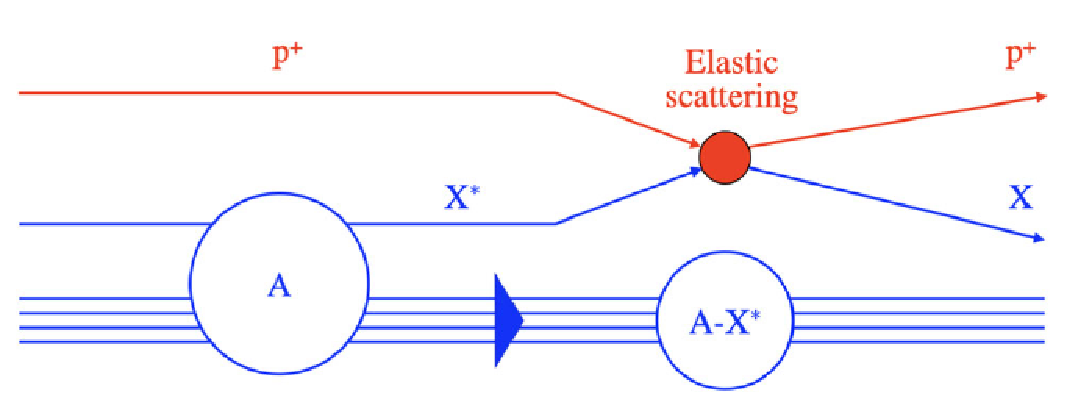
\includegraphics[width=\linewidth]{QFS_Reaction_Scheme}
	\caption{Schematic diagram of a QFS reaction induced by a proton p$^+$ on a nucleus A via elastic scattering off the virtual constituent particle X$^*$. Three real particles are generated in the final state: the scattered proton p$^+$, the knock-out cluster X and the spectator nuclear fragment (A-X$^*$). Reprinted figure from Ref. \cite{panin_quasi-free_2021}}
	\label{fig:QFS_Scheme}
\end{figure}

\subsection{The Modern Era: Inverse Kinematics and Exotic Nuclei}

A transformative leap occurred in the 21st century with the advent of inverse kinematics \gls{QFS} using radioactive ion beams (RIBs) and hydrogen targets. As comprehensively reviewed by Panin et al. (2021) \cite{panin_quasi-free_2021}, modern \gls{QFS} experiments at facilities such as RIKEN, GSI/FAIR, and FRIB utilize high-energy beams of neutron- or proton-rich nuclei impinging on proton-rich targets. The resulting reactions—such as (p,2p), (p,pn), or (p,p$\alpha$)—enable the study of short-lived and exotic systems far from stability, including halo nuclei, nuclei near the neutron drip line, and those within the so-called "island of inversion."

These experiments exploit complete kinematic reconstruction techniques, coincident $\gamma$-ray detection, and high-resolution tracking of all final-state particles. This allows the identification of orbital angular momentum (\emph{l}) of removed nucleons via momentum distributions, providing a model-independent probe of nuclear shell structure. Moreover, inverse kinematics \gls{QFS} has facilitated the spectroscopy of unbound states, the quantification of short-range correlations (SRCs), and insights into clustering phenomena in light and medium-mass nuclei.


\subsection{Benchmark and Current Frontiers}

\gls{QFS} today occupies a unique position among reaction mechanisms, bridging single-particle and correlated many-body dynamics. Benchmarked by decades of electron-induced \gls{QFS} data, modern (p, 2p)/(p, pn) measurements are now used to:

\begin{itemize}
	\item Test shell evolution in neutron-rich isotopes.
	\item Quantify spectroscopic factors and their reduction (quenching).
	\item Investigate SRCs in asymmetric nuclear matter.
	\item Map the extent of the island of inversion.
	\item Explore the nature of unbound and resonant nuclear states.
\end{itemize}

Theoretical advancements, notably the eikonal DWIA and relativistic frameworks, allow consistent comparisons between experiment and shell-model or ab initio structure predictions. Future developments—such as the integration of machine learning in reaction theory, or the use of polarized beams and targets—promise even finer resolution of nuclear substructure.


%
% Please note that
% \begin{center}
%   \textbf{\large this package and template are not official for FCT/NOVA}.
% \end{center}



% \printbibliography[heading=subbibliography, segment=\therefsegment, title={\bibname\ for chapter~\thechapter}]
